\documentclass[11pt,letterpaper]{article}
\usepackage[lmargin=1in,rmargin=1in,tmargin=1in,bmargin=1in]{geometry}
\usepackage{../style/homework}
\usepackage{../style/commands}
\setbool{quotetype}{false} % True: Side; False: Under
\setbool{hideans}{true} % Student: True; Instructor: False

\newcommand{\xor}{\,\underline{\vee}\,}

% Logical Circuits
\usepackage{circuitikz}
\usetikzlibrary{shapes.gates.logic.US,shapes.gates.logic.IEC}

% -------------------
% Content
% -------------------
\begin{document}

\homework{2: Due 09/12}{I am very seldom interested in applications. I am more interested in the elegance of a problem. Is it a good problem, an interesting problem?}{Claude Shannon}

% Problem 1
\problem{10} Often, one encounters expressions along the lines, ``This happens, unless this.'' In symbolic form, we could write this as, ``$P$ happens, unless $Q$.'' Most often, what is meant by this is, ``if $\neg Q$, then $P$.'' That is, ``$P$ unless $Q$'' means $\neg Q \to P$. 
	\begin{enumerate}[(a)]
	\item Consider the statement, ``Payment is due on fifth of the month, unless it is a weekend.'' Rewrite this statement in ``if\dots then'' form.  
	\item Write the negation of ``Payment is due on fifth of each month, unless it is a weekend'' as a complete English sentence. 
	\item Is payment not being due a sufficient condition for the fifth being the weekend? Explain. 
	\item Is the fifth of the month being a weekend sufficient for payment not being due? Explain. 
	\end{enumerate}



\newpage



% Problem 2
\problem{10} In everyday speech, ``this or that'' could mean, ``this, that, or both'' or it could mean, ``this, that, but not both.'' Both interpretations are common. ``Mathematical OR'' \textit{always} allows the possibility for both, i.e. $P \vee Q$ is true if $P$ is true, $Q$ is true, or both $P$ and $Q$ are true. It would be advantageous to have an ``exclusive or'' for logical expressions. Define ``mathematical exclusive or'' to be $P \xor Q$; that is, $P \xor Q$ is true when exactly one of $P$, $Q$ is true. 
	\begin{enumerate}[(a)]
	\item Give the logic table for $P \xor Q$
	\item Using a logic table, show that $P \xor Q \equiv (P \wedge \neg Q) \vee (\neg P \wedge Q)$.
	\item Without computing $P \xor Q \iff (P \wedge \neg Q) \vee (\neg P \wedge Q)$, determine whether this proposition is a tautology. Explain. 
	\item Use (b) to find a logical expression for $\neg (P \xor Q)$ in terms of $P$'s, $Q$'s, $\neg$'s, $\wedge$'s, and $\vee$'s; that is, find a `rule' for determining how to negate $P \xor Q$. `Simplify' your expression as much as possible. 	
	\end{enumerate}



\newpage



% Problem 3
\problem{10} We can use Boolean representations of circuits to simplify circuits and reduce the amount of wire, chips, etc. required. Consider the circuit below:
	\[
	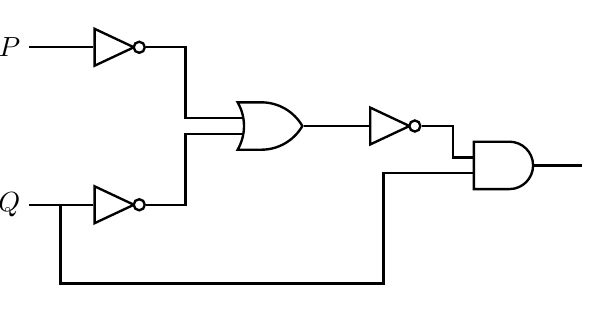
\begin{tikzpicture}
	\node (p) at (0,2) {\hspace{-0.5cm}$P$};
	\node (q) at (0,0) {\hspace{-0.5cm}$Q$};
	
	\node[not gate US, draw, line width= 0.03cm] at (1,2) (not1) {};
	\node[not gate US, draw, line width= 0.03cm] at (1,0) (not2) {};
	\node[not gate US, draw, line width= 0.03cm] at (4.5,1) (not3) {};
	\node[or gate US, draw, line width= 0.03cm] at (3,1) (or1) {};
	\node[and gate US, draw, line width= 0.03cm] at (6,0.5) (and1) {};
	
	\draw[line width= 0.03cm] (p) |- (not1.input);
	\draw[line width= 0.03cm] (q) |- (not2.input);
	
	\draw[line width= 0.03cm] (not1.output) -- ([xshift=0.5cm]not1.output) |- (or1.input 1);
	\draw[line width= 0.03cm] (not2.output) -- ([xshift=0.5cm]not2.output) |- (or1.input 2);
	
	\draw[line width= 0.03cm] (or1.output) |- (not3.input);
	\draw[line width= 0.03cm] (not3.output) -- ([xshift=0.4cm]not3.output) |- (and1.input 1);
	\draw[line width= 0.03cm] (q) |- (0.4,0) |- (0.4,-1) |- (4.5,-1) |- (and1.input 2);
	
	\draw[line width= 0.03cm] (and1.output) |- ([xshift=0.6cm]and1.output);
	\end{tikzpicture}
	\]

\begin{enumerate}[(a)]
\item Find the logical expression corresponding to the given circuit.
\item `Simplify' the logical expression from (a).
\item Sketch the circuit from (b).
\end{enumerate}



\newpage



% Problem 4
\problem{10} Draw a circuit diagram corresponding to the logical expression below and construct its input/output table.
	\[
	\neg (P \vee \neg Q) \wedge (P \vee Q)
	\]



\newpage



% Problem 5
\problem{10} Watch at least one of the following videos:
	\begin{itemize}
	\item \href{https://www.youtube.com/watch?v=QZwneRb-zqA&ab_channel=SebastianLague}{Exploring How Computers Work}
	\item \href{https://www.youtube.com/watch?v=I0-izyq6q5s&ab_channel=SebastianLague}{How Do Computers Remember?}
	\end{itemize}
Then as thoroughly as possible, comment on what you observed and learned from the video. Be sure to remark as much as possible on how these videos connect to the course content. 


\end{document}